\appendix
\setcounter{equation}{0}
\setcounter{figure}{0}
\renewcommand{\theequation}{A.\arabic{equation}}
\renewcommand\thefigure{A.\arabic{figure}}

\section{Online appendix}
\label{sec:Appendix}

This is the Online Appendix for the paper:

\begin{center}
Rodríguez-Sánchez P, van Nes EH, Scheffer M. \textit{Neutral competition boosts chaos in food webs}.
\end{center}

\subsection{Generalized multispecies predation models}
\label{subsec:GeneralizedModels}

\subsubsection{General properties of predation models}
\label{subsubsec:GeneralPropertiesOfPredation}

Most predation models based on differential equations follow a structure like this:
%
\begin{eqnarray}
\label{eq:CommonStructure}
	\begin{cases}
	P'(t) = Growth(P) - Predation(P,C)
	\\
	C'(t) = -Loss(C) + GrossGrowth(P,C)
	\end{cases}
\end{eqnarray}
%
where $P$ represents the biomass of the prey population, and $C$ the biomass of the consumer/predator population. The functional dependencies have been explicitly written in order to remark the fact that the coupling of the system happens via the $Predation$ and $GrossGrowth$ terms.

It is important to note that, in models like this, all deaths at the prey's level are due to predation. All deaths caused by predation are invested in consumer's growth. Therefore the following relation must be true:
%
\begin{equation}
\label{eq:InnerEnergyFlow}
	GrossGrowth(P,C) = e \cdot Predation(P,C)
\end{equation}
%
where $e$ represents the efficiency of the energy transfer process. Equation \eqref{eq:InnerEnergyFlow}, when plugged into \eqref{eq:CommonStructure}, yields:
%
\begin{equation}
\label{eq:AllEnergyFlow}
	e P'(t) + C'(t) = e \cdot Growth(P) - Loss(C)
\end{equation}
%
Equation \eqref{eq:AllEnergyFlow} allows us to think of our system as an open system from the point of view of thermodynamics. Here $Growth$ is the only source of the system, and $Loss$ is the only sink (see figure \ref{fig:EnergyFlow}). All the energy exchange due to predation stays inside the system, so predation can be considered a closed subsystem.

\begin{figure}[H]
	\begin{center}
		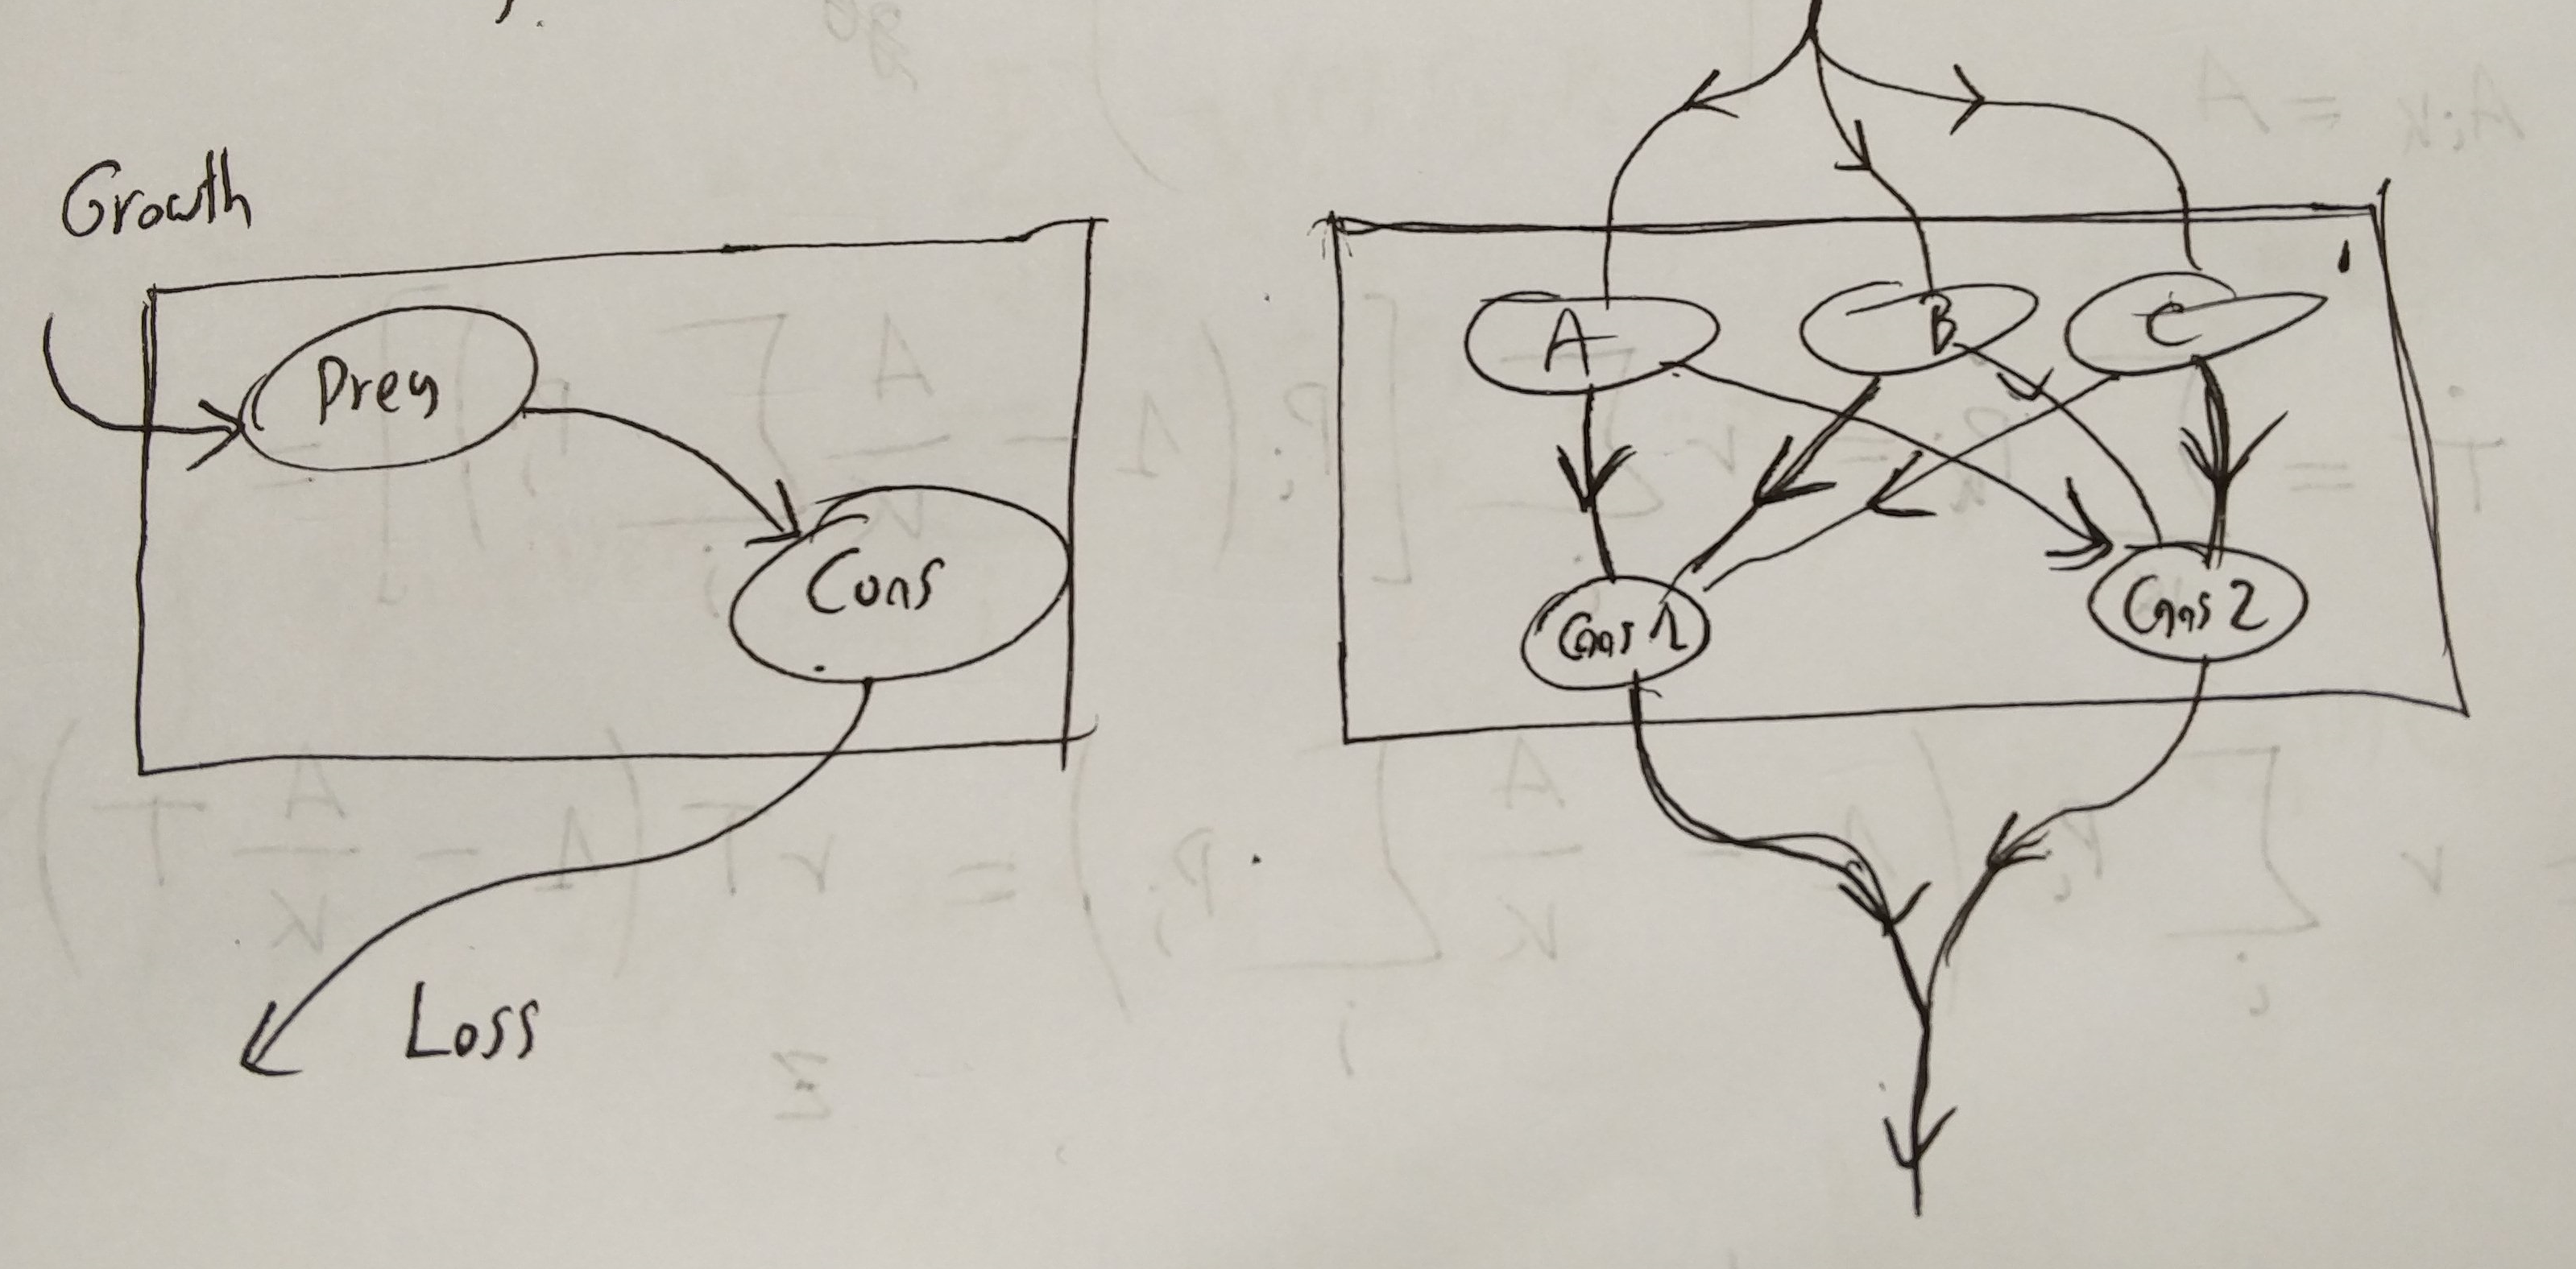
\includegraphics[width=0.25\columnwidth]{energyflow.png}
	\end{center}
	\caption{Plot showing the energy flow in our class of systems.}
	\label{fig:EnergyFlow}
\end{figure}

We can generalize this basic structure to multispecies, two trophic levels systems. First, we'll go back to equation \eqref{eq:CommonStructure} and just add more rows:
%
\begin{eqnarray}
\label{eq:CommonStructureMulti}
	\begin{cases}
	P_i'(t) = Growth_i(P) - Predation_i(P_i,C) & : i = 1..n_P
	\\
	C_j'(t) = -Loss_j(C_j) + GrossGrowth_j(P,C_j) & : j = 1..n_C
	\end{cases}
\end{eqnarray}
%
where now $i$ runs from $1$ to the number of prey $n_P$ and $j$ from $1$ to the number of consumers $n_C$. Here, we've used $P_i$ to denote the population of the prey labeled by $i$, and $P$ for the vector containing all prey populations. Notice that while the $Growth$ term can involve competition (and thus, depends on the whole vector $P$), the $Loss$ term for species $j$ depends only in the population of that species (i.e.: $C_j$), regardless of the rest.

Requiring once again our predation to be fully invested in consumer's growth, we find the following generalization of equation \eqref{eq:InnerEnergyFlow}:
%
\begin{equation}
\label{eq:InnerEnergyFlowMulti}
	\sum_{j = 1}^{n_C} GrossGrowth_j(P,C_j) = \sum_{i = 1}^{n_P} e_i \cdot Predation_i(P_i,C)
\end{equation}
%
Using \eqref{eq:InnerEnergyFlowMulti} and \eqref{eq:CommonStructureMulti}, it is easy to prove that the multispecies generalization of \eqref{eq:AllEnergyFlow} is:
%
\begin{equation}
\label{eq:AllEnergyFlowMulti}
	\sum_{i = 1}^{n_P} e_i P_i'(t) + \sum_{j = 1}^{n_C} C_j'(t) = \sum_{i = 1}^{n_P} e_i \cdot Growth_i(P) - \sum_{j = 1}^{n_C} Loss_j(C_j)
\end{equation}
%
The intuitive interpretation is, again, that the only sinks and sources of energy in our systems are the total $Loss$ and $Growth$.

Restriction \eqref{eq:InnerEnergyFlowMulti} (or equivalently, \eqref{eq:AllEnergyFlowMulti}) can be used to generalize realistic functional forms for the coupling terms.

\subsubsection{Lotka-Volterra equations}
\label{subsubsec:LotkaVolterra}

The most basic model of predation is the Lotka-Volterra system of equations:
%
\begin{eqnarray}
\label{eq:LotkaVolterra}
	\begin{cases}
	P'(t) = r P - g P C
	\\
	C'(t) = - l C + e g C P
	\end{cases}
\end{eqnarray}
%
where $r$ represents the growth rate of the prey, $g$ the grazing rate of the predator against the prey, $l$ the loss rate of the predator and $e$ the efficiency conversion factor.

It is trivial to prove that the Lotka-Volterra model satisfies the requirements shown in subsection \ref{subsubsec:GeneralPropertiesOfPredation}.

\subsubsection{Multispecies Lotka-Volterra equations}
\label{subsubsec:LotkaVolterraMulti}

Lotka-Volterra equations can be generalized to a model with multiple species by noting that each prey will be affected by all consumers, and each consumer will be affected by all prey. In order to code the strength of this interactions, we introduce the matrix $S$, whose element $S_{ji}$ gives the strength of the coupling of consumer $j$ and prey $i$. As a consequence, for prey dynamics this matrix is scanned row-wise, while for predators it is scanned column-wise. The generalized system looks like:
%
\begin{eqnarray}
\label{eq:LotkaVolterraMulti}
	\begin{cases}
	P_i'(t) = r_i P_i - P_i \sum_{j = 1}^{n_C} g_j S_{ji} C_j & : i = 1..n_P
	\\
	C_j'(t) = - l_j C_j +  g_j e_j C_j \sum_{i = 1}^{n_P} S_{ji} P_i  & : j = 1..n_C
	\end{cases}
\end{eqnarray}
%
The fulfillment of condition \eqref{eq:InnerEnergyFlowMulti} is again easily proven.

In this model, all terms can grow without boundaries. This is not only unrealistic, but also creates some problems from the sole point of view of mathematical stability.

\subsubsection{Rosenzweig-MacArthur model}
\label{subsubsec:Rosenzweig-MacArthur}
The Rosenzweig-MacArthur predator-prey model improves the previous model by adding boundaries to the terms' dependency on the prey population. This is achieved by encapsulating $P$ inside saturating functions. In particular, the growth rate and the grazing rate $r$ now depend on $P$ (see equation \eqref{eq:RosMac2levels} and compare it with \eqref{eq:LotkaVolterra}).
%
\begin{eqnarray}
\label{eq:RosMac2levels}
	\begin{cases}
	P'(t) = r(P) P - g(P) P C
	\\
	C'(t) = - l C + e g(P) C P
	\end{cases}
\end{eqnarray}
%
Once again, condition \eqref{eq:InnerEnergyFlow} is trivially fulfilled independently of the functional form of $r(P)$ and $g(P)$. If both functions are chosen appropriately, we avoid unbounded growths. Typically, $r(P)$ and $g(P)$ are chosen so they generate a logistic growth and a Holling type II saturation response when plugged into \eqref{eq:RosMac2levels}. In mathematical terms, this means choosing $r(P) = r_0 \left(1 - \frac{P}{K} \right)$ and $g(P) = \frac{g_0}{P+H}$ (for more information see, for instance, \citet{Edelstein-Keshet}). After making this choices, our system takes its classical form:
%
\begin{eqnarray}
\label{eq:RosMac2classic}
	\begin{cases}
	P'(t) =  r P \left( 1 - \frac{P}{K} \right) - g C \frac{P}{P + H}
	\\
	C'(t) = - l C + e g C \frac{P}{P + H}
	\end{cases}
\end{eqnarray}
%

\subsubsection{Multispecies Rosenzweig-MacArthur model}
\label{subsubsec:Rosenzweig-MacArthurMulti}

Noticing the similarities between equations \eqref{eq:LotkaVolterra} and \eqref{eq:RosMac2levels}, the latter can be generalized in the same fashion as we did to obtain \eqref{eq:LotkaVolterraMulti}, yielding:
%
\begin{eqnarray}
\label{eq:RosMacMulti}
	\begin{cases}
	P_i'(t) = r_i(P) P_i - P_i \sum_{j = 1}^{n_C} g_j(P) S_{ji} C_j & : i = 1..n_P
	\\
	C_j'(t) = - l_j C_j +  g_j(P) e_j C_j \sum_{i = 1}^{n_P} S_{ji} P_i  & : j = 1..n_C
	\end{cases}
\end{eqnarray}
%
Written like this, it is easy to see that the condition \eqref{eq:InnerEnergyFlowMulti} is fulfilled.

Regarding the proper functional forms of $r_i(P)$ and $g_j(P)$, our growth term has to take into account both the inter and intraspecific competition. This can be easily modelled by choosing:
%
\begin{equation}
\label{eq:r}
	r_i(P) = r_i \left( 1 - \sum_{k=1}^{n_P} A_{ik} P_k \right)
\end{equation}
%
where the matrix elements $A_{ik}$ account for the intensity of the competition caused by species $k$ on species $i$. Thus, non-diagonal elements account for interspecific competition, and diagonal ones for intraspecific competition.

We hypothesize that the grazing rates corresponding to predator $j$, that is, $g_j(P)$, follow a Holling type II functional response dependent on the total consumption of prey by predator $j$:
%
\begin{eqnarray}
\label{eq:g}
	g_j(P) = \frac{g_j}{\sum_{i=1}^{n_P} S_{ji} P_i + H_j}
\end{eqnarray}
%

\subsubsection{Summary}
\label{subsubsec:SummaryPredation}

\begin{table}[H]
\label{tab:SummaryPredation}
	\begin{center}
		\resizebox{\columnwidth}{!}{
			\begin{tabular}{|c|c|c|} \hline
				 & Two species & Multispecies \\
				\hline
				Lotka-Volterra & $\begin{cases}P'(t) = r P - g P C\\ C'(t) = - l C + e g C P\end{cases}$ & $\begin{cases} P_i'(t) = r_i P_i - P_i \sum_{j = 1}^{n_C} g_j S_{ji} C_j \\ C_j'(t) = - l_j C_j +  g_j e_j C_j \sum_{i = 1}^{n_P} S_{ji} P_i \end{cases}$ \\
				\hline
				Rosenzweig-MacArthur & $\begin{cases}P'(t) = r(P) P - g(P) P C\\C'(t) = - l C + e g(P) C P\end{cases}$ & $\begin{cases} P_i'(t) = r_i(P) P_i - P_i \sum_{j = 1}^{n_C} g_j(P) S_{ji} C_j \\ C_j'(t) = - l_j C_j +  g_j(P) e_j C_j \sum_{i = 1}^{n_P} S_{ji} P_i \end{cases}$  \\
			\hline  \end{tabular}}
	\end{center}
	\caption{Summary table with the different types of predation models studied. Written this way, the parallelisms are obvious. In multispecies models, the index $i$ runs from $1$ to $n_P$, and $j$ from $1$ to $n_C$. The functional forms of $r_i(P)$ and $g_j(P)$ are given in equations \eqref{eq:r} and \eqref{eq:g}. In the present paper we used the Rosenzweig-MacArthur multispecies model, that is, the one in the lower right corner.}
\end{table}

\subsection{Chaos detection}
\label{subsec:ChaosDetection}
In the exploratory phase of this research three parallel approaches to chaos detection were followed: Lyapunov exponents estimation  \citep{Strogatz1994}, Gottwald - Melbourne \textit{0-1} test \citep{Gottwald2009} and visual inspection. Despite differences in the exact probabilities, the three of them led us to the same qualitative conclusions (see figure \ref{fig:AllContours}). We found the Gottwald - Melbourne test to be the fastest and most reliable of all.

\begin{figure}[H]
	\begin{center}
		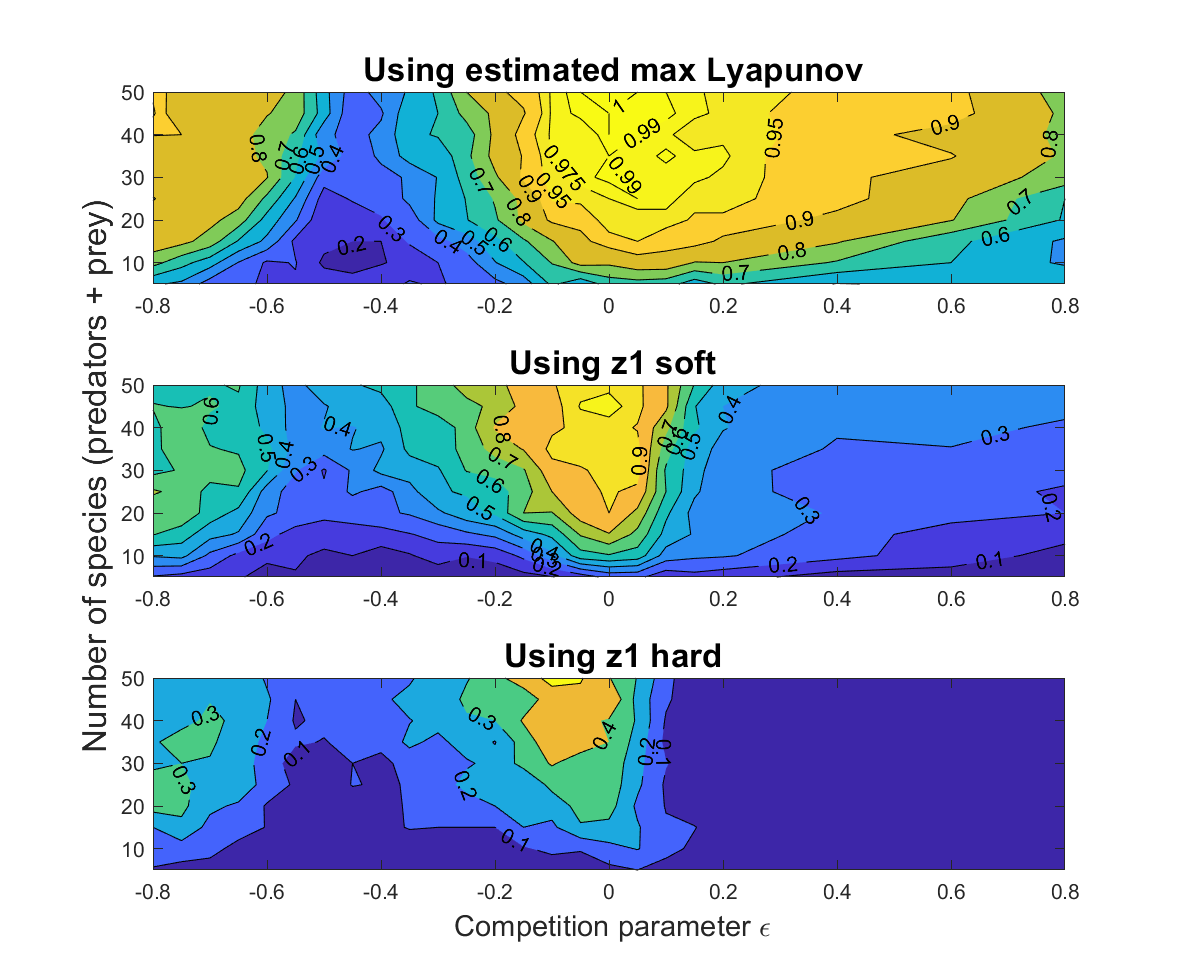
\includegraphics[width=1\columnwidth]{contours_all.png}
	\end{center}
	\caption{Performing the same analysis with different chaos detection algorithms we found different numerical results. The upper panel used the estimation of the maximum Lyapunov exponent as a test for chaoticity. The second and third used the z1 Gottwald - Melbourne test, with different degrees of tolerance. In particular, \textit{z1 soft} is more prone to classify complicated cycles as chaos, and \textit{z1 hard} is more likely to throw indecisive results. Even for the most conservative test (\textit{z1 hard}), the qualitative conclusions (that is, that chaos happens more frequently in the vicinity of neutral competition) still hold.}
	\label{fig:AllContours}
\end{figure}

\subsubsection{Melbourne-Gottwald 0-1 test in a nutshell}
\label{subsubsec:z1test}
The 0-1 test for chaos is designed for distinguishing between regular and chaotic dynamics in deterministic systems. It works directly with the observed time series, so a prior knowledge of the underlying dynamics is not required (as long as we know that they are deterministic).

This short section is more a motivation than a rigorous proof. A minimal, intuitive approach to the method will be outlined. For a detailed, complete explanation please refer to \citet{Gottwald2009}.

First, we have to use one of our time series of observations $\phi_k$ to build the functions:
%
\begin{eqnarray}
\label{eq:z1}
	\begin{cases}
	p_n(\theta) = \sum_{k=1}^n \phi_k cos(k \theta)
	\\
	q_n(\theta) = \sum_{k=1}^n \phi_k sin(k \theta)
	\end{cases}
\end{eqnarray}
%
Using Euler's formula both equations can be given a more compact form:
%
\begin{equation}
\label{eq:z1complex}
z_n(\theta) = p_n(\theta) + i q_n(\theta) = \sum_{k=1}^n \phi_k e^{i k \theta}
\end{equation}
%
In the complex plane, $e^{i k \theta}$ represents a unit vector pointing in the direction $k \theta$. So each observation in our time series can be understood as the size of a step, being $k \theta$ its direction (see table \ref{tab:Summands}).

\begin{table}[H]
\begin{center}
\begin{tabular}{|c|c|c|c|c|c|}
\hline
k & 0 & 1 & 2 & 3 & ...\\
\hline
$k \theta$ & 0 & $\frac{\pi}{6}$ & $\frac{2\pi}{6}$ & $\frac{\pi}{2}$ & ...\\
\hline
$e^{i k \theta}$ & 
\begin{tikzpicture} \draw[->, ultra thick, red,  arrows={-latex}] (0,0) -- (1,0); \end{tikzpicture} & 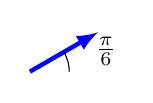
\begin{tikzpicture} \draw[->, ultra thick, blue,  arrows={-latex}]  (0,0) -- (0.866,0.5); \draw (0.5,0) arc (0:30:0.5) node[] at (15:1) {$\frac{\pi}{6}$}; \end{tikzpicture} & 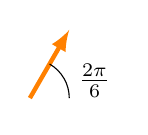
\begin{tikzpicture} \draw[->, ultra thick, orange,  arrows={-latex}]  (0,0) -- (0.5,0.866); \draw (0.5,0) arc (0:60:0.5) node[] at (15:0.85) {$\frac{2\pi}{6}$}; \end{tikzpicture} & 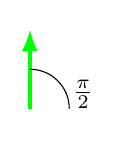
\begin{tikzpicture} \draw[->, ultra thick, green,  arrows={-latex}]  (0,0) -- (0,1); \draw (0.5,0) arc (0:90:0.5) node[] at (15:0.7){$\frac{\pi}{2}$}; \end{tikzpicture} & ... \\
\hline
$\phi_k$ & 2 & 1 & 0.5 & 0.25 & ...\\
\hline
$\phi_k e^{i k \theta}$ & 
\begin{tikzpicture} \draw[->, ultra thick, red,  arrows={-latex}]  (0,0) -- (2,0); \end{tikzpicture} & 
\begin{tikzpicture} \draw[->, ultra thick, blue,  arrows={-latex}]  (0,0) -- (0.866,0.5); \end{tikzpicture} & 
\begin{tikzpicture} \draw[->, ultra thick, orange,  arrows={-latex}]  (0,0) -- (0.25,0.433); \end{tikzpicture} & 
\begin{tikzpicture} \draw[->, ultra thick, green,  arrows={-latex}]  (0,0) -- (0,0.25); \end{tikzpicture} & ... \\
\hline
\end{tabular}
\end{center}
\caption{\label{tab:Summands} Example showing a step by step geometrical construction of the elements inside the summation operator in equation \eqref{eq:z1complex}. In this example we use a time series whose first elements are $\phi_j = \left\lbrace 2, 1, 0.5, 0.25, ...\right\rbrace$. The parameter $\theta$ has been set to $\frac{\pi}{6}$.}
\end{table}

Adding up the elements in table \ref{tab:Summands} as indicated by equation \eqref{eq:z1complex} can be interpreted geometrically as vector addition, i.e., performing one "step" after another (see figure \ref{fig:Sum}).

\begin{figure}[H]
\begin{center}
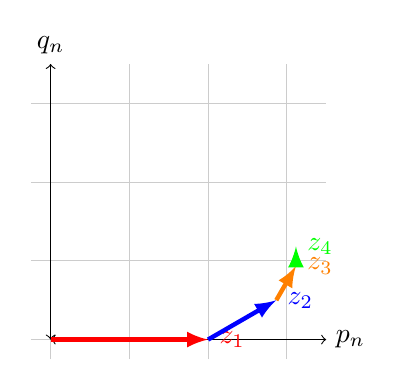
\begin{tikzpicture}
	% Grid
  	\draw[thin,gray!40] (-0.25,-0.25) grid (3.5,3.5);

  	% Axes
    \draw[<->] (0,0)--(3.5, 0) node[right]{$p_n$};
  	\draw[<->] (0,0)--(0, 3.5) node[above]{$q_n$};

	% Data
  	\draw[->, ultra thick, red,  arrows={-latex}]  (0,0) -- (2,0) node[right]{$z_1$};
  	\draw[->, ultra thick, blue,  arrows={-latex}]  (2,0) -- (2.866,0.5) node[right]{$z_2$};
  	\draw[->, ultra thick, orange,  arrows={-latex}]  (2.866,0.5) -- (3.116,0.933) node[right]{$z_3$};
  	\draw[->, ultra thick, green,  arrows={-latex}]  (3.116,0.933) -- (3.116,1.183) node[right]{$z_4$};

\end{tikzpicture}
\end{center}
\caption{\label{fig:Sum} Geometrical calculation of $z_1, z_2, z_3$ and  $z_4$ for $\phi_j = \left\lbrace 2, 1, 0.5, 0.25, ...\right\rbrace$ and $\theta = \frac{\pi}{6}$.}
\end{figure}

With this picture in mind, it is easy to understand the kind of paths that different types of time series will give rise to (see figure \ref{fig:z1Path}). Constant time series generate cyclic paths (polygons) or pseudocyclic paths (polygons that do not close after a first round). Periodic or pseudoperiodic time series generate periodic or pseudoperiodic paths (note that the summand in \eqref{eq:z1complex} becomes then the product of two periodic/pseudoperiodic functions). Random time series generate brownian-motion-like paths. Provided that our system is deterministic, the apparent stochasticity of our observed time series is a strong indicator of chaos.

\begin{figure}
	\begin{center}
		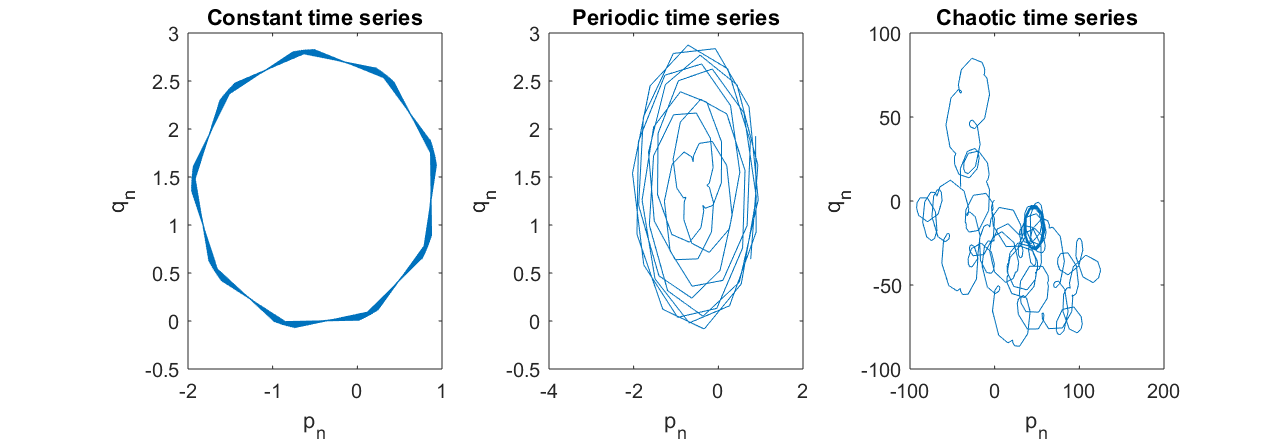
\includegraphics[width=1\columnwidth]{z1.png}
	\end{center}
	\caption{First and second panels show the paths generated by the z1 test when applied to constant and periodic time series. The third panel shows the case with a chaotic time series (notice the different scale). While in the first two cases the paths remain inside a bounded domain, in the chaotic case the path drifts away from the starting point in a brownian-motion-like fashion.}
	\label{fig:z1Path}
\end{figure}

The case of an underlying chaotic time series is the only one that generates a path that doesn't stay inside a bounded domain around the starting point. The z1 test uses the mean square displacement as a measure of this drift. The system is considered to be chaotic if the square displacement keeps growing for large times. If, on the contrary, it stays bounded, the test will consider the system not chaotic.


\subsection{Extra figures}
\label{subsec:ExtraFigures}

\subsubsection{Multispecies predator-prey network}
\label{subsubsec:MultispeciesPPNetwork}
\begin{figure}[H]
	\begin{center}
		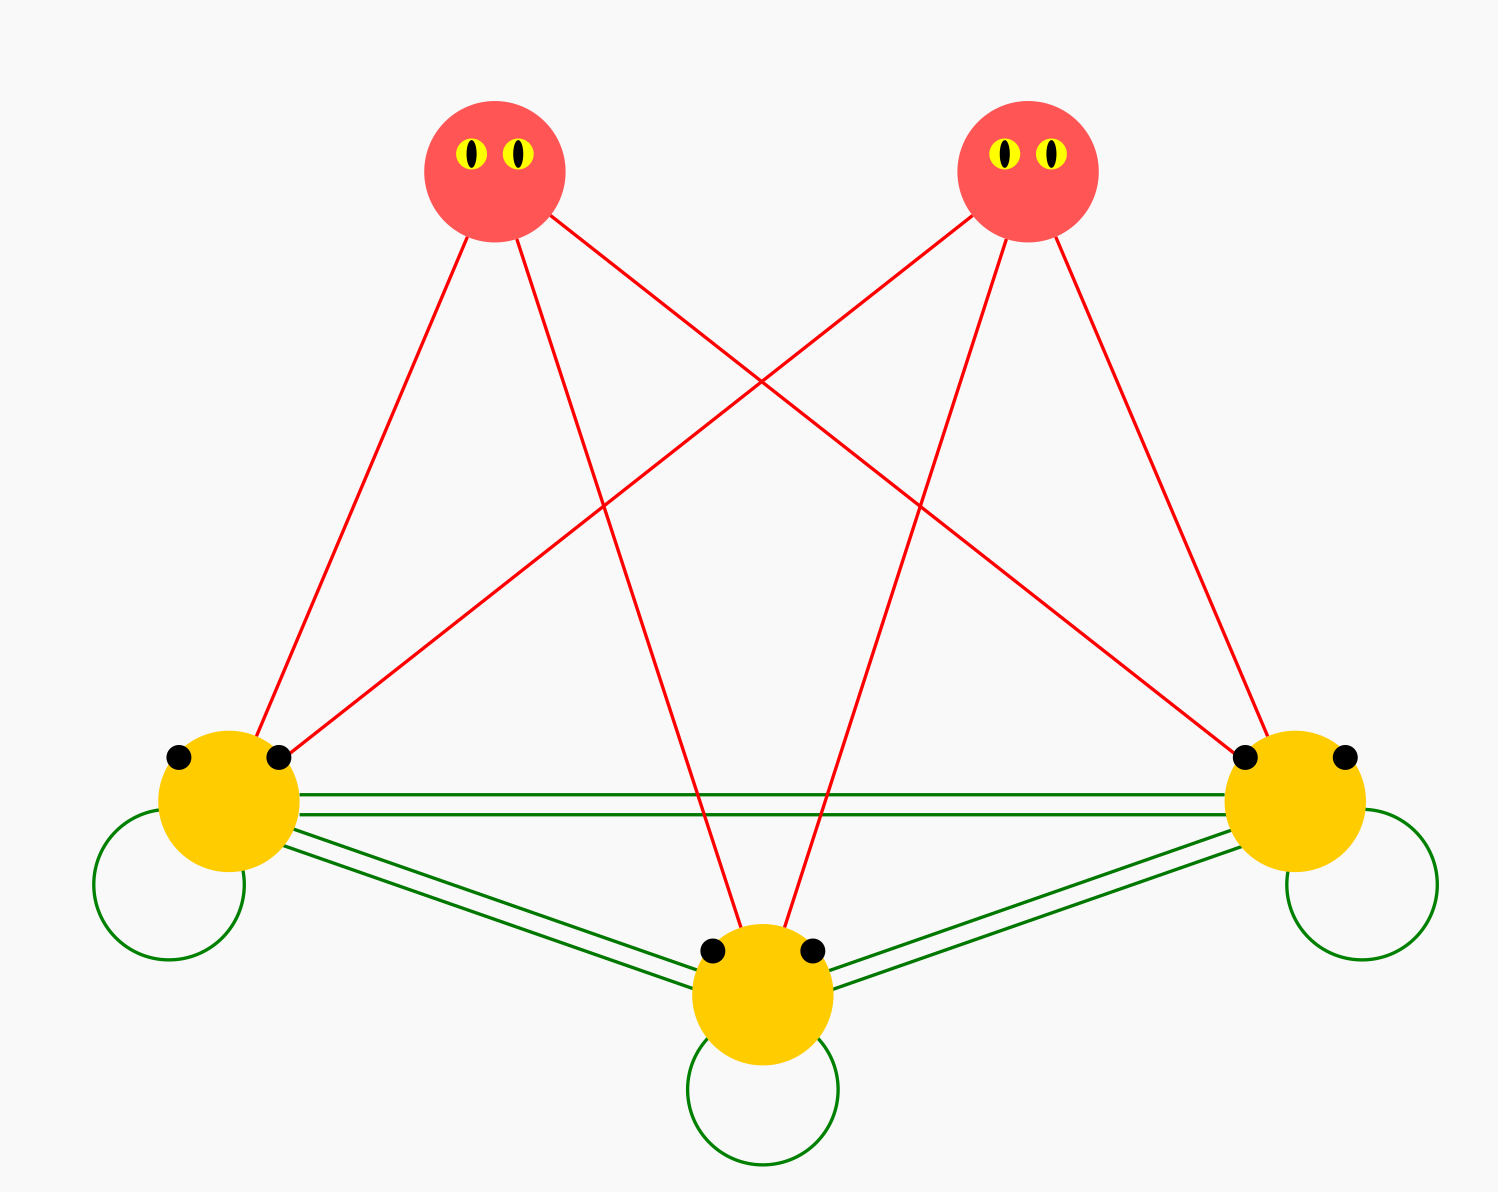
\includegraphics[width=0.5\columnwidth]{net.png}
	\end{center}
	\caption{Example with $2$ consumers and $3$ prey. Each one of the red links represents a predation interaction (coded in the matrix of predator preference coefficients, $ S $). Each green link represents a competition interaction (coded in the matrix of competition coefficients, $ A $). The closed green loops are related with carrying capacity (diagonal elements of $ A $) interpreted here as intra-species competition.}
	\label{fig:Network}
\end{figure}

\subsubsection{Probabilities grouped by number of species}
\label{subsubsec:AllProbabilities}
\begin{figure}[H]
	\begin{center}
		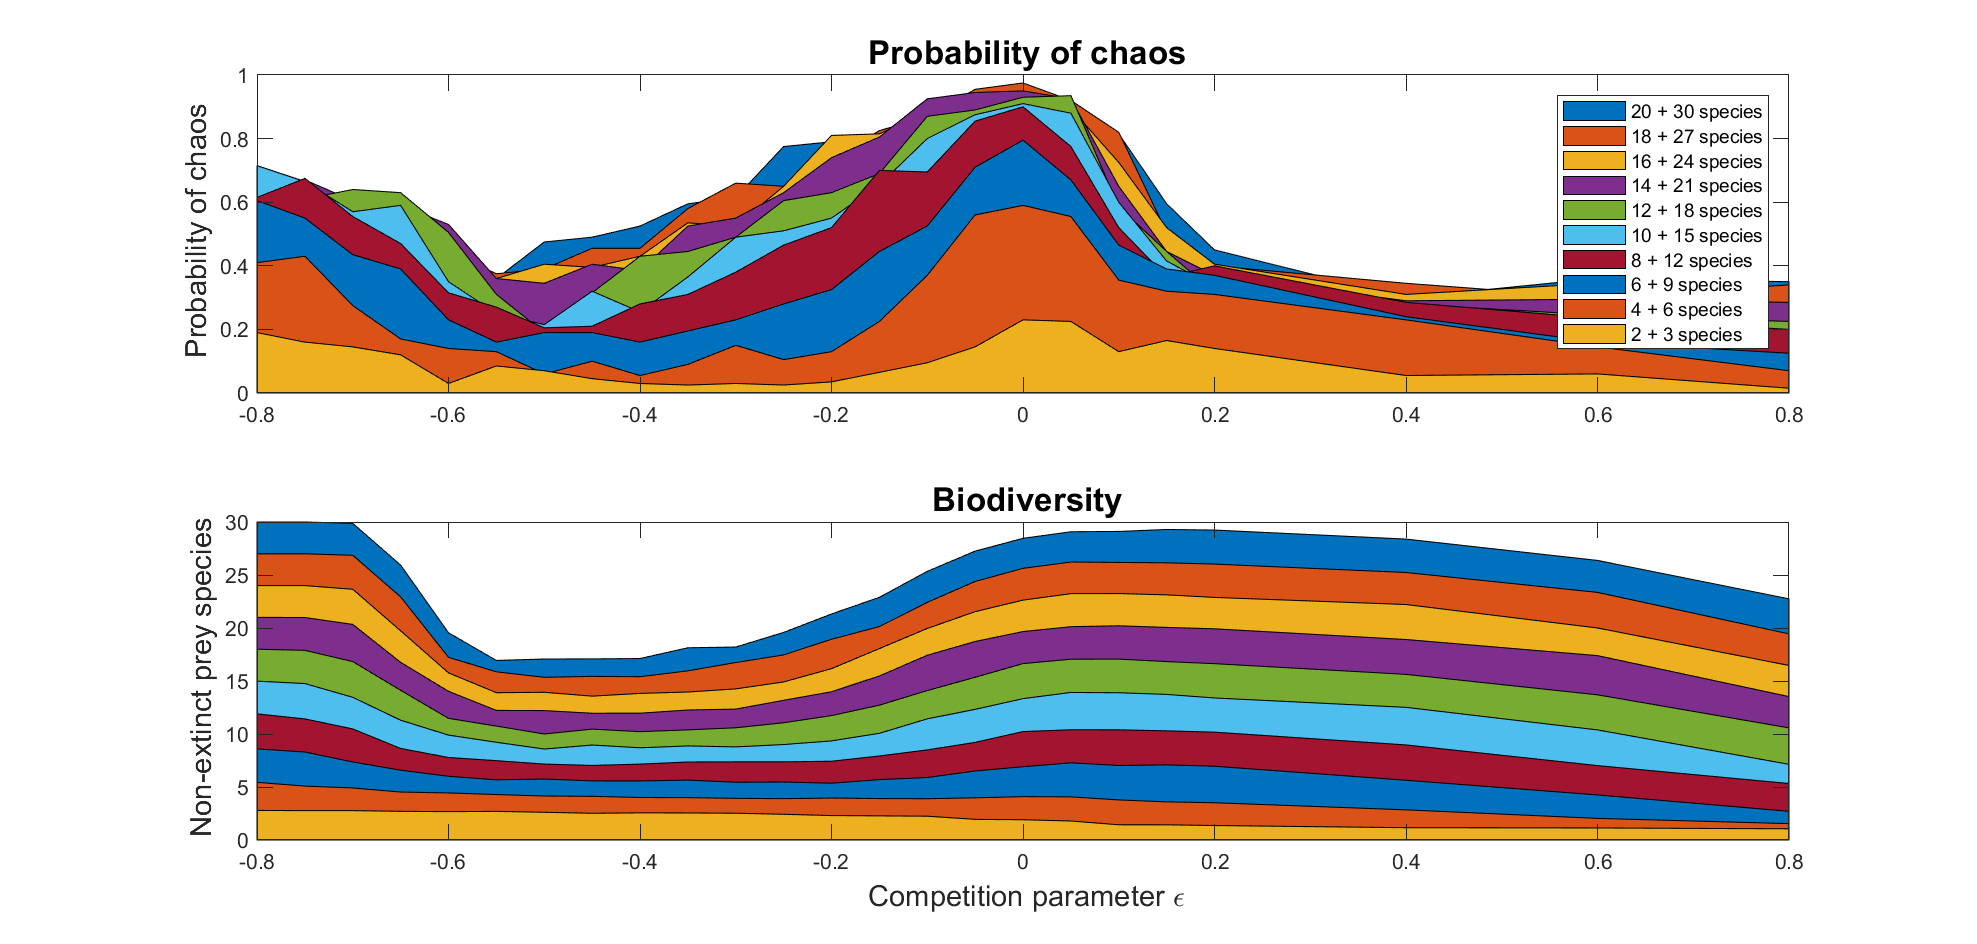
\includegraphics[width=1\columnwidth]{results_all.png}
	\end{center}
	\caption{Summary of the results of the whole set of simulations. The competition parameter $\epsilon$ is on the horizontal axis. The estimated probability of chaos is represented on the vertical one. Each panel corresponds to an ecosystem with a different number of interacting species. The exact number is shown in each box, as number of predators + number of prey.}
	\label{fig:AllProbabilities}
\end{figure}

\subsubsection{Biodiversity measurements}
\label{subsubsec:BiodiversityFigs}

For each simulation, a biodiversity index was estimated as the number of prey species whose population was higher than a minimum threshold of $\bioThreshold$ $mg$ $l^{-1}$, averaged respective to time.

\begin{figure}[H]
	\begin{center}
		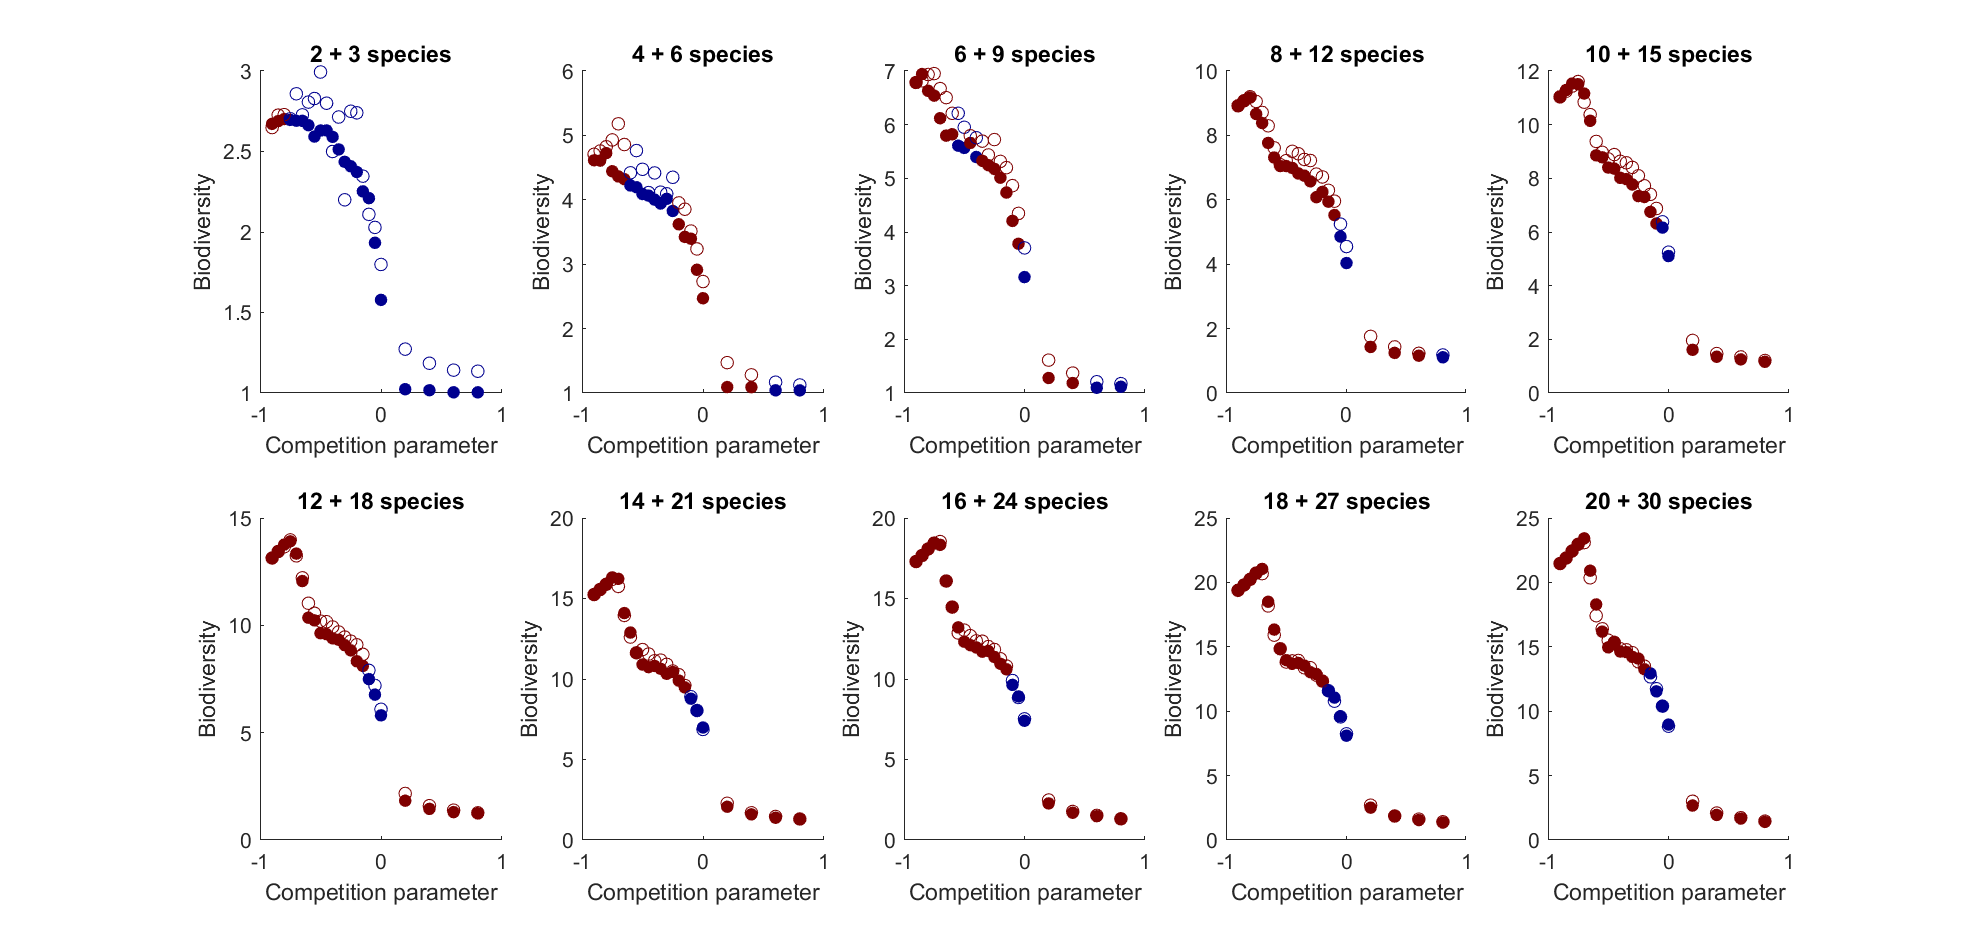
\includegraphics[width=1\columnwidth]{biod_split_by_chaos.png}
	\end{center}
	\caption{Average prey biodiversity vs. competition parameter. Each panel shows a food network of a different size. For each value of the competition parameter, 200 randomly drawn ecosystems were simulated. The dashed line shows the average number of prey species of these 200 simulations. The white circles represent the average prey biodiversity of those simulations who had chaotic dynamics, the black circles represent the same for non-chaotic dynamics. The relative area of the white to the black circles represents the ratio of chaotic to regular dynamics.}
	\label{fig:BiodSplitByChaos}
\end{figure}

\begin{figure}[H]
	\begin{center}
		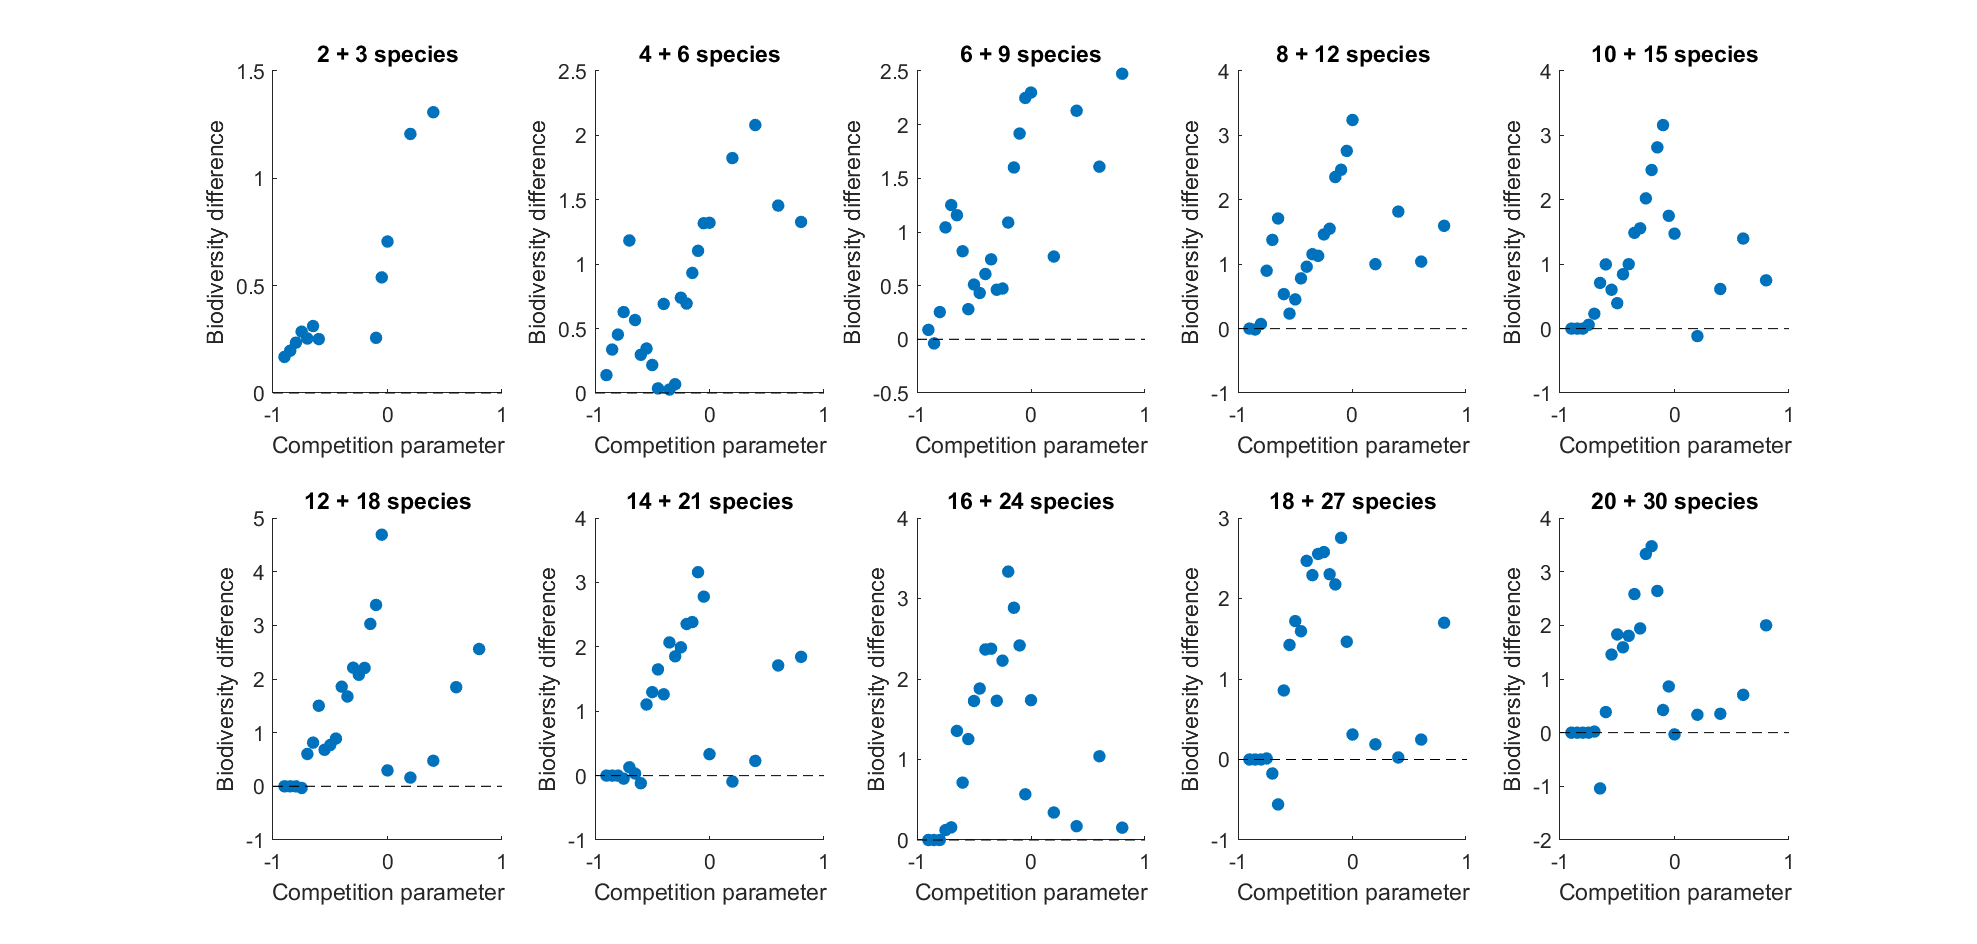
\includegraphics[width=1\columnwidth]{biod_split_by_chaos_diff.png}
	\end{center}
	\caption{Each set of simulated ecosystems was grouped by competition parameter $\epsilon$ and then classified as chaotic or regular. The difference in average prey biodiversities for the chaotic and the regular case is plotted here vs. the competition parameter. Cases where the ratio chaotic-regular was outside the range 20 \% - 80 \% are marked in blue.}
	\label{fig:BiodSplitByChaosDiff}
\end{figure}

\begin{figure}[H]
	\begin{center}
		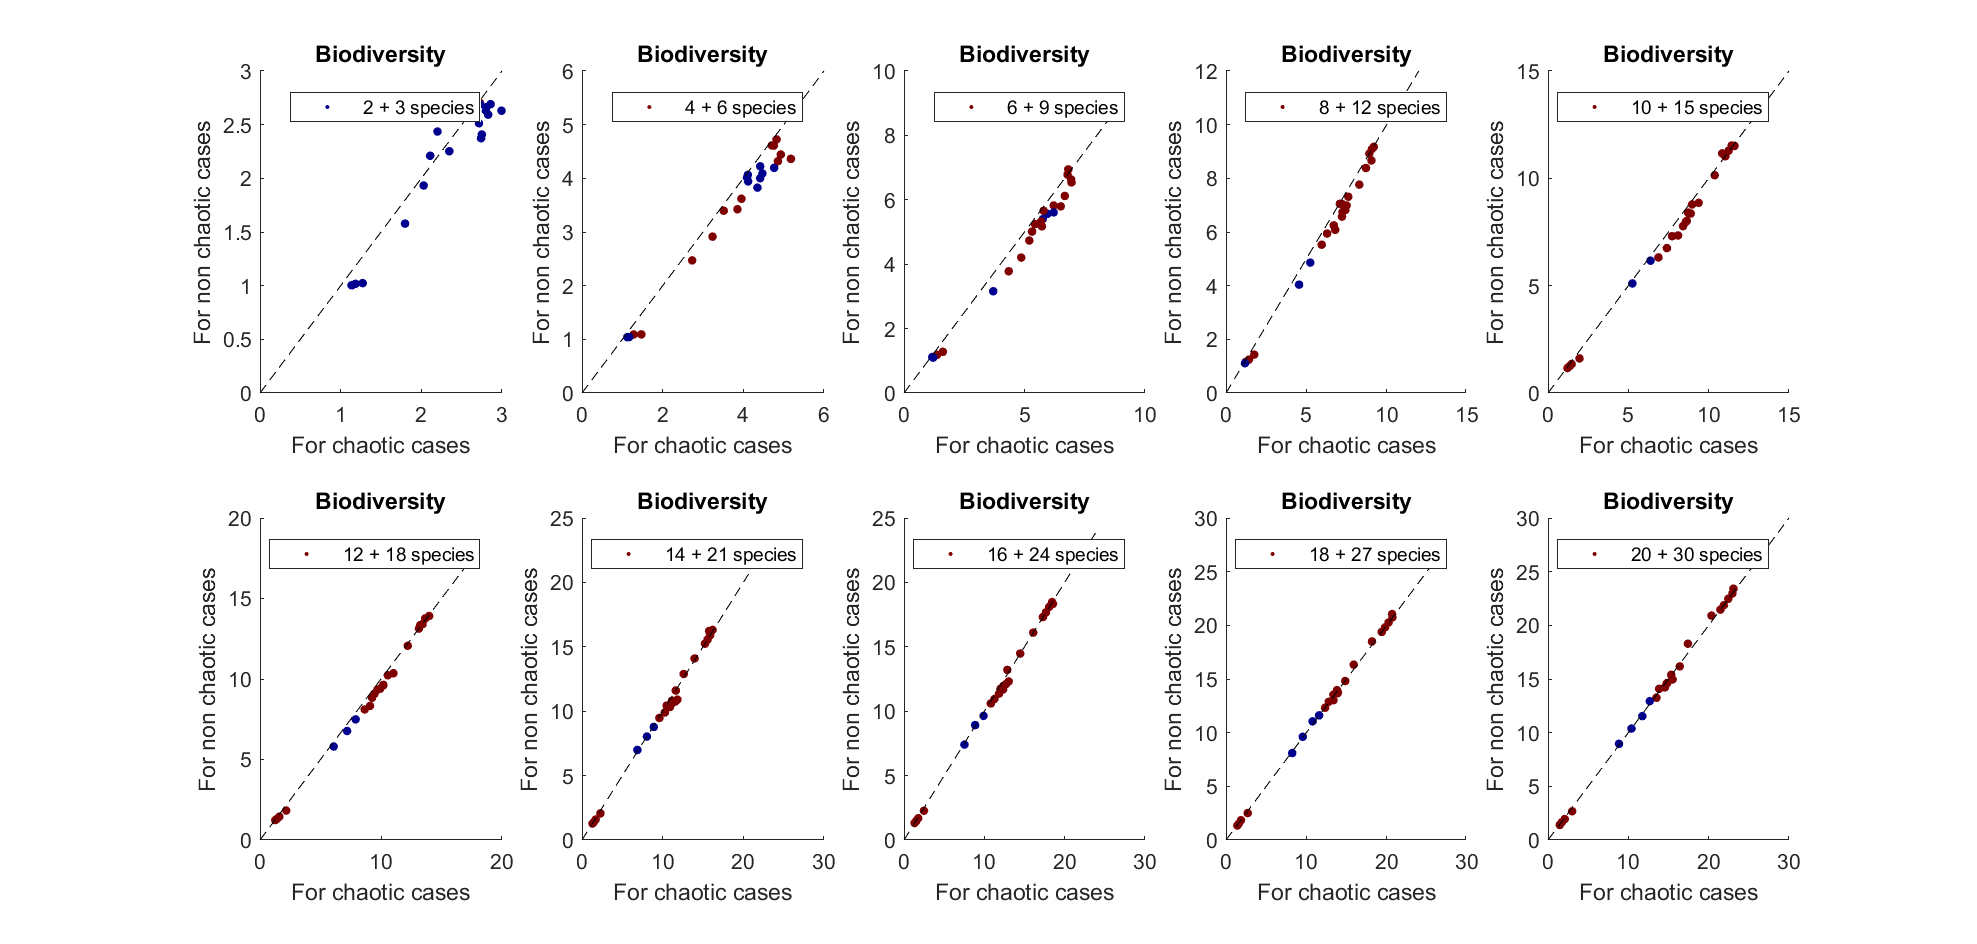
\includegraphics[width=1\columnwidth]{biod_chaos_vs_regular.png}
	\end{center}
	\caption{Each set of simulated ecosystems was grouped by competition parameter $\epsilon$ and then classified as chaotic or regular. The average prey biodiversity of the regular cases is plotted here vs. the average prey biodiversity of the chaotic cases. Cases where the ratio chaotic-regular was outside the range 20 \% - 80 \% are marked in blue.}
	\label{fig:BiodChaosVsRegular}
\end{figure}

\begin{figure}[H]
	\begin{center}
		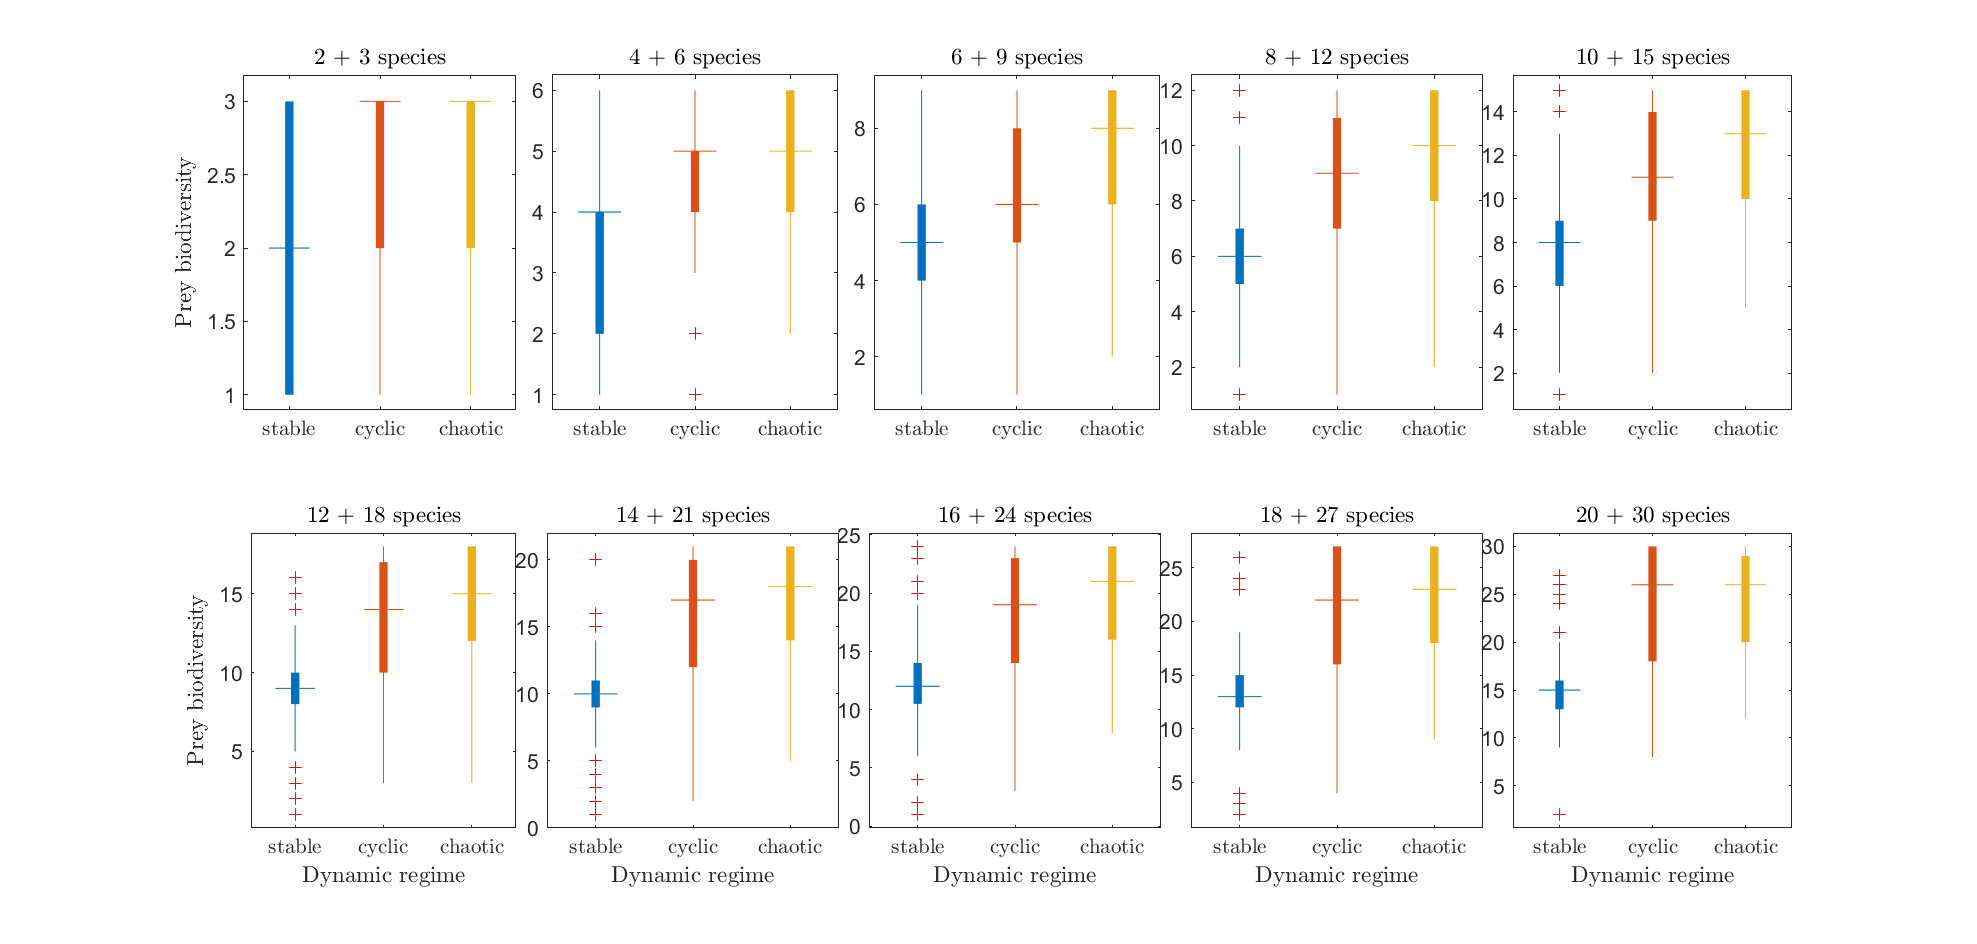
\includegraphics[width=1\columnwidth]{biod_box_and_whisker.png}
	\end{center}
	\caption{Box and whisker plot of the prey biodiversity, after being classified as regular or chaotic.}
	\label{fig:BiodBoxAndWhisker}
\end{figure}

\subsubsection{Flow chart}
\label{subsubsec:FlowChart}
In the spirit of reproducible research we made available all the analysis code used to draw our conclusions. Any interested researcher can clone it from a \textit{GitHub} repository \citep{Rodriguez-Sanchez-code-neuchaos} and, executing a single script, reproduce all our simulations and figures. This figure shows schematically what this script does:

\begin{figure}[H]
	\begin{center}
		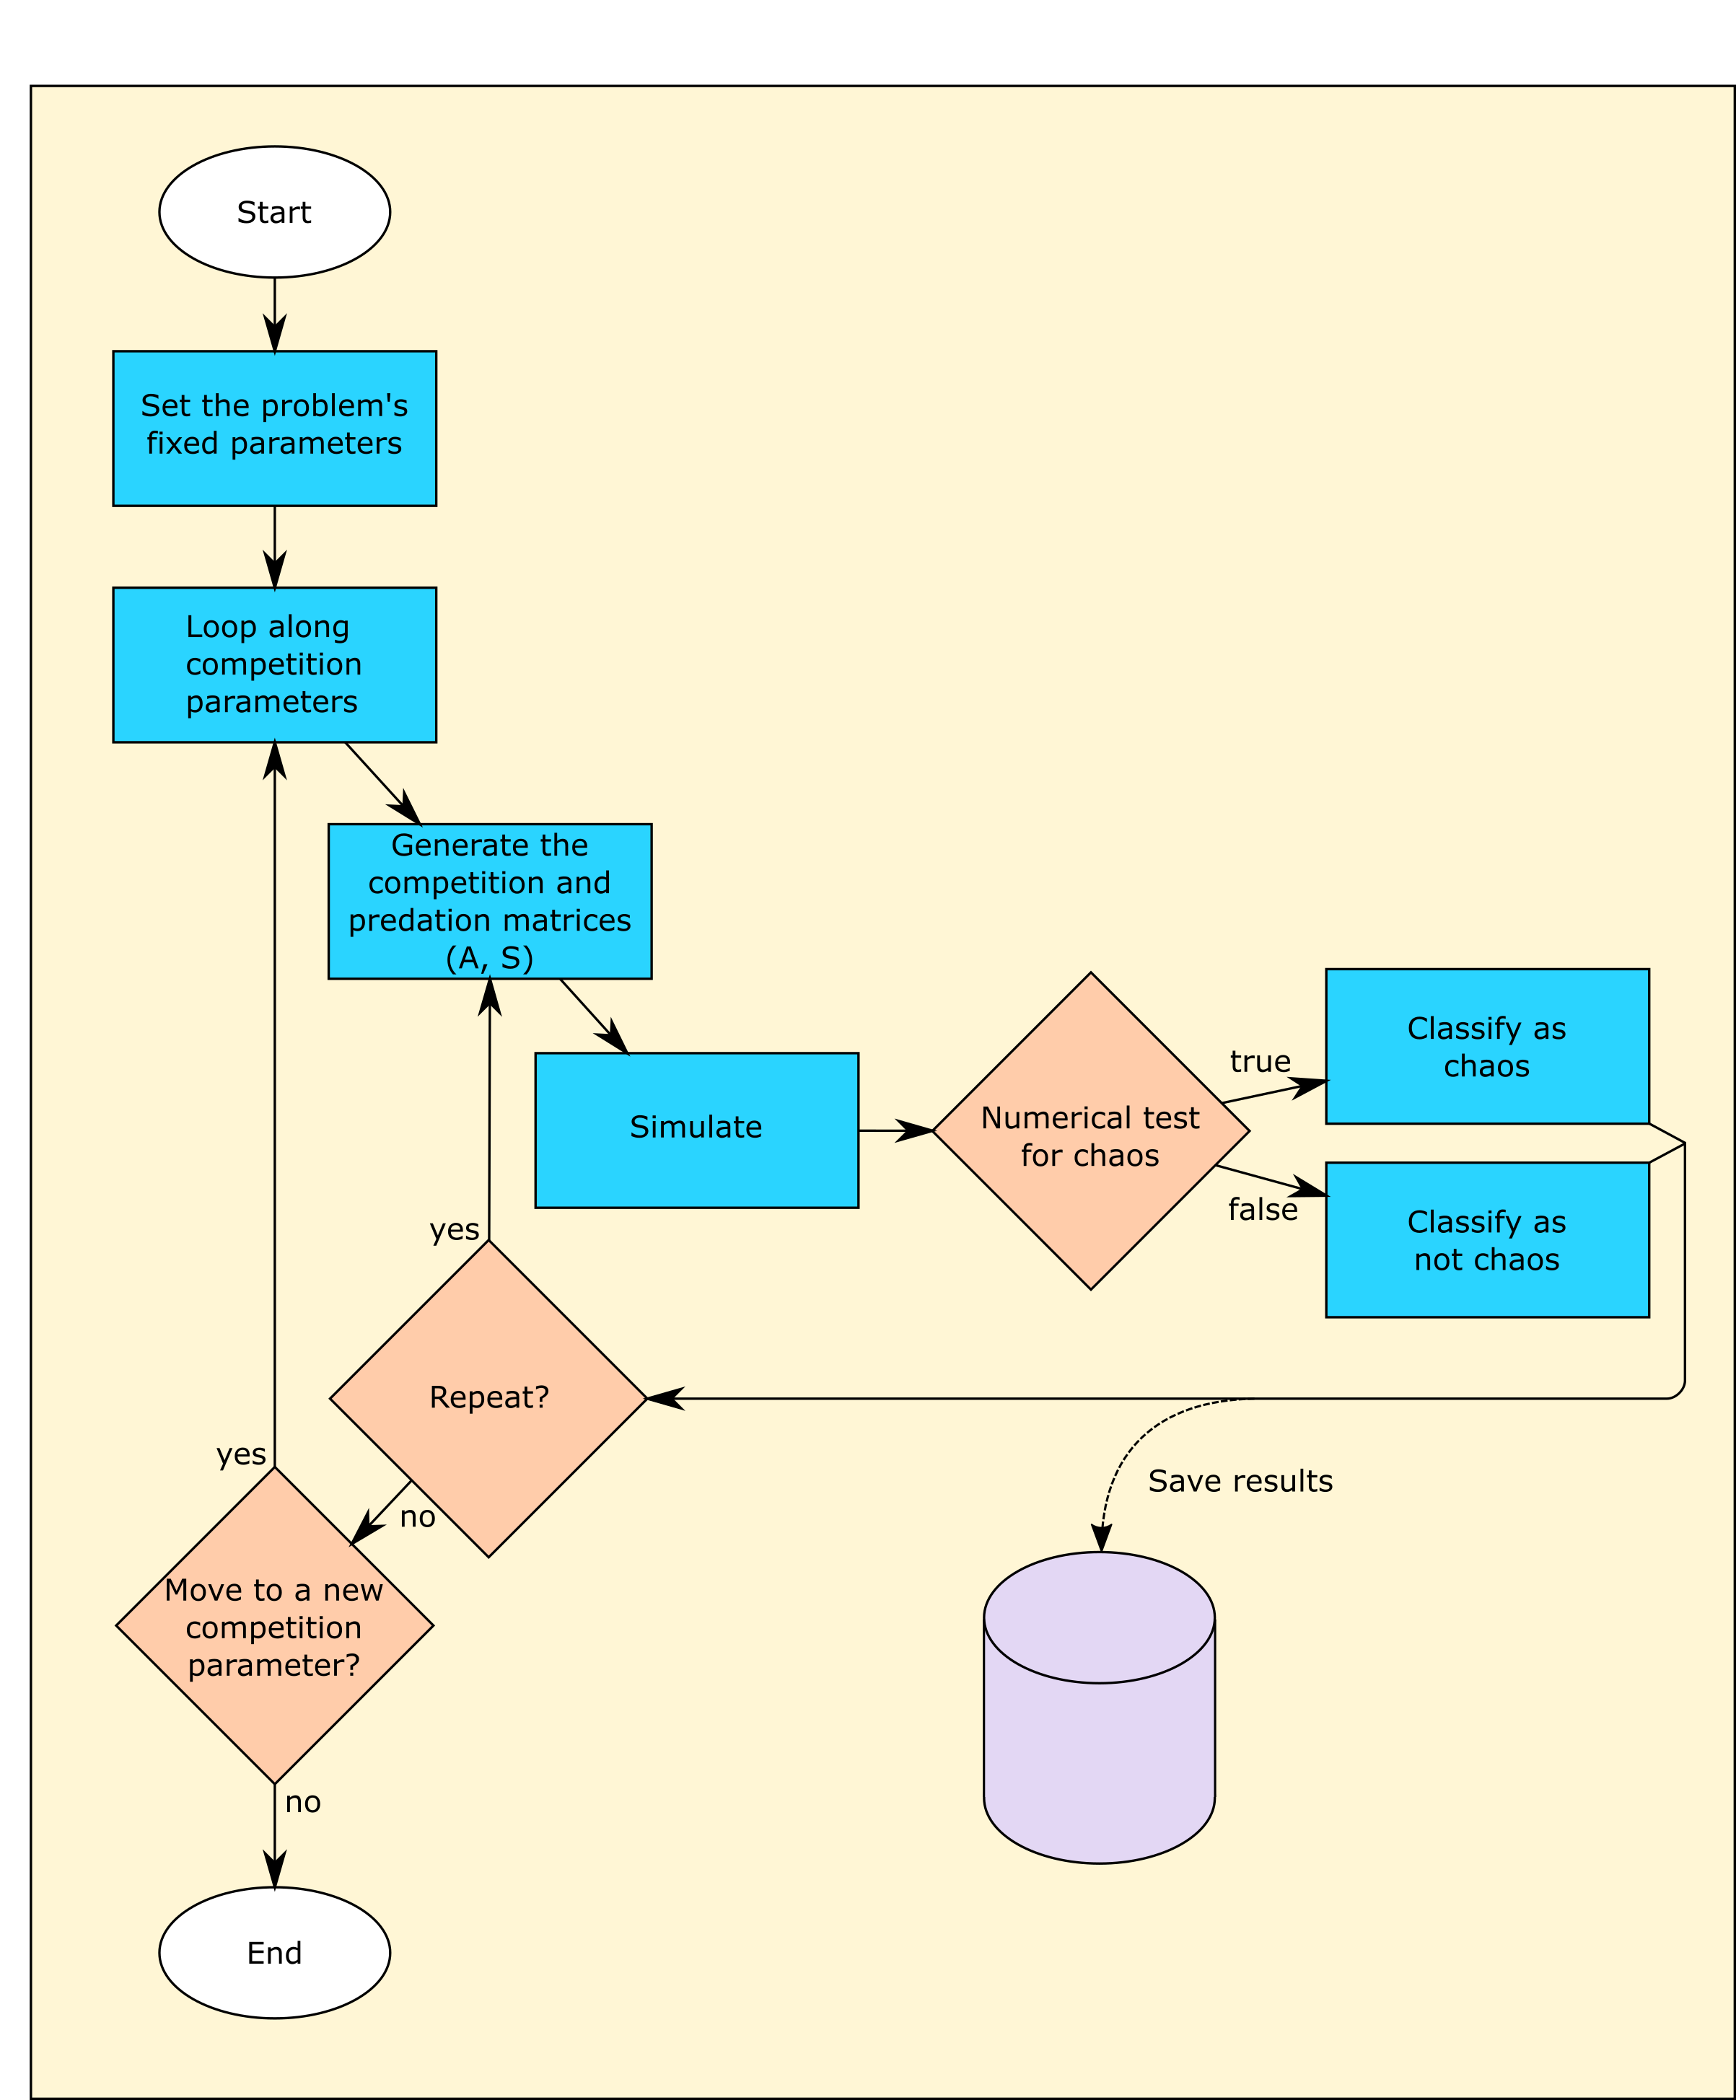
\includegraphics[width=0.8\columnwidth]{flow_chart.png}
	\end{center}
	\caption{Flow chart describing the numerical experiment. The source code is available at \textit{\texttt{https://doi.org/10.5281/zenodo.1319590}}.}
	\label{fig:FlowChart}
\end{figure}
